% Options for packages loaded elsewhere
\PassOptionsToPackage{unicode}{hyperref}
\PassOptionsToPackage{hyphens}{url}
%
\documentclass[
  12pt,
]{article}
\usepackage{amsmath,amssymb}
\usepackage{lmodern}
\usepackage{ifxetex,ifluatex}
\ifnum 0\ifxetex 1\fi\ifluatex 1\fi=0 % if pdftex
  \usepackage[T1]{fontenc}
  \usepackage[utf8]{inputenc}
  \usepackage{textcomp} % provide euro and other symbols
\else % if luatex or xetex
  \usepackage{unicode-math}
  \defaultfontfeatures{Scale=MatchLowercase}
  \defaultfontfeatures[\rmfamily]{Ligatures=TeX,Scale=1}
\fi
% Use upquote if available, for straight quotes in verbatim environments
\IfFileExists{upquote.sty}{\usepackage{upquote}}{}
\IfFileExists{microtype.sty}{% use microtype if available
  \usepackage[]{microtype}
  \UseMicrotypeSet[protrusion]{basicmath} % disable protrusion for tt fonts
}{}
\makeatletter
\@ifundefined{KOMAClassName}{% if non-KOMA class
  \IfFileExists{parskip.sty}{%
    \usepackage{parskip}
  }{% else
    \setlength{\parindent}{0pt}
    \setlength{\parskip}{6pt plus 2pt minus 1pt}}
}{% if KOMA class
  \KOMAoptions{parskip=half}}
\makeatother
\usepackage{xcolor}
\IfFileExists{xurl.sty}{\usepackage{xurl}}{} % add URL line breaks if available
\IfFileExists{bookmark.sty}{\usepackage{bookmark}}{\usepackage{hyperref}}
\hypersetup{
  pdftitle={Ticketing and Turnout: The Participatory Consequences of Low-Level Police Contact},
  hidelinks,
  pdfcreator={LaTeX via pandoc}}
\urlstyle{same} % disable monospaced font for URLs
\usepackage[margin=1in]{geometry}
\usepackage{longtable,booktabs,array}
\usepackage{calc} % for calculating minipage widths
% Correct order of tables after \paragraph or \subparagraph
\usepackage{etoolbox}
\makeatletter
\patchcmd\longtable{\par}{\if@noskipsec\mbox{}\fi\par}{}{}
\makeatother
% Allow footnotes in longtable head/foot
\IfFileExists{footnotehyper.sty}{\usepackage{footnotehyper}}{\usepackage{footnote}}
\makesavenoteenv{longtable}
\usepackage{graphicx}
\makeatletter
\def\maxwidth{\ifdim\Gin@nat@width>\linewidth\linewidth\else\Gin@nat@width\fi}
\def\maxheight{\ifdim\Gin@nat@height>\textheight\textheight\else\Gin@nat@height\fi}
\makeatother
% Scale images if necessary, so that they will not overflow the page
% margins by default, and it is still possible to overwrite the defaults
% using explicit options in \includegraphics[width, height, ...]{}
\setkeys{Gin}{width=\maxwidth,height=\maxheight,keepaspectratio}
% Set default figure placement to htbp
\makeatletter
\def\fps@figure{htbp}
\makeatother
\setlength{\emergencystretch}{3em} % prevent overfull lines
\providecommand{\tightlist}{%
  \setlength{\itemsep}{0pt}\setlength{\parskip}{0pt}}
\setcounter{secnumdepth}{5}
\usepackage{rotating}
\usepackage{setspace}
\usepackage{booktabs}
\usepackage{longtable}
\usepackage{array}
\usepackage{multirow}
\usepackage{wrapfig}
\usepackage{float}
\usepackage{colortbl}
\usepackage{pdflscape}
\usepackage{tabu}
\usepackage{threeparttable}
\usepackage{threeparttablex}
\usepackage[normalem]{ulem}
\usepackage{makecell}
\usepackage{xcolor}
\ifluatex
  \usepackage{selnolig}  % disable illegal ligatures
\fi

\title{Ticketing and Turnout: The Participatory Consequences of Low-Level Police Contact}
\author{}
\date{\vspace{-2.5em}May 04, 2022}

\begin{document}
\maketitle

\pagenumbering{gobble}
\pagebreak

\pagenumbering{arabic}
\doublespacing

\begin{figure}[H]

{\centering 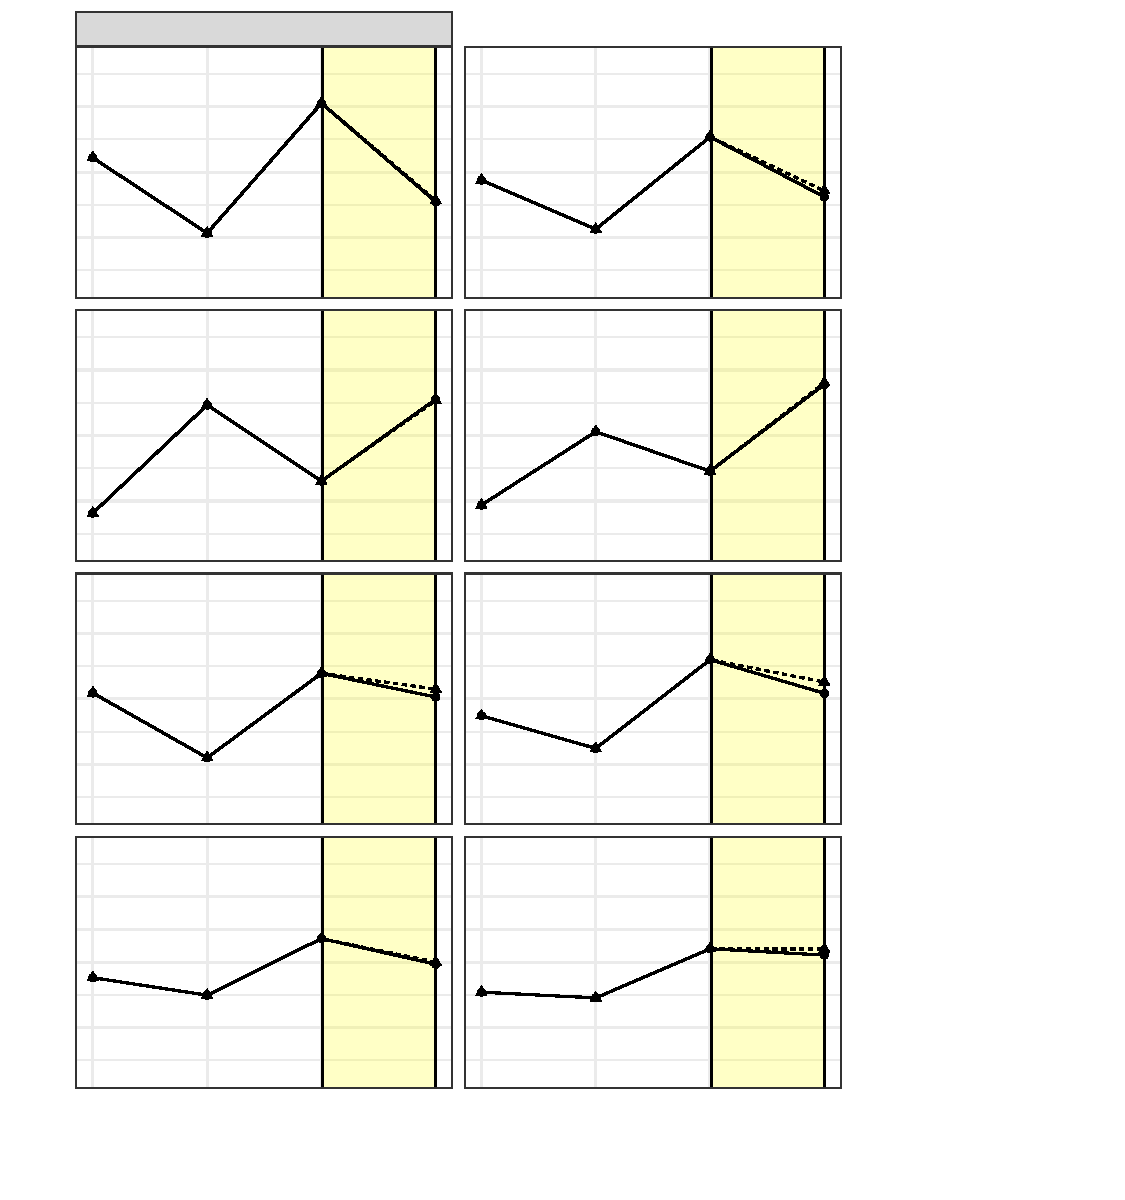
\includegraphics{compile_files/figure-latex/did-primary-1} 

}

\caption{\label{fig:did-1}Effect of Being Ticketed on Turnout}\label{fig:did-primary}
\end{figure}

\begin{figure}[H]

{\centering 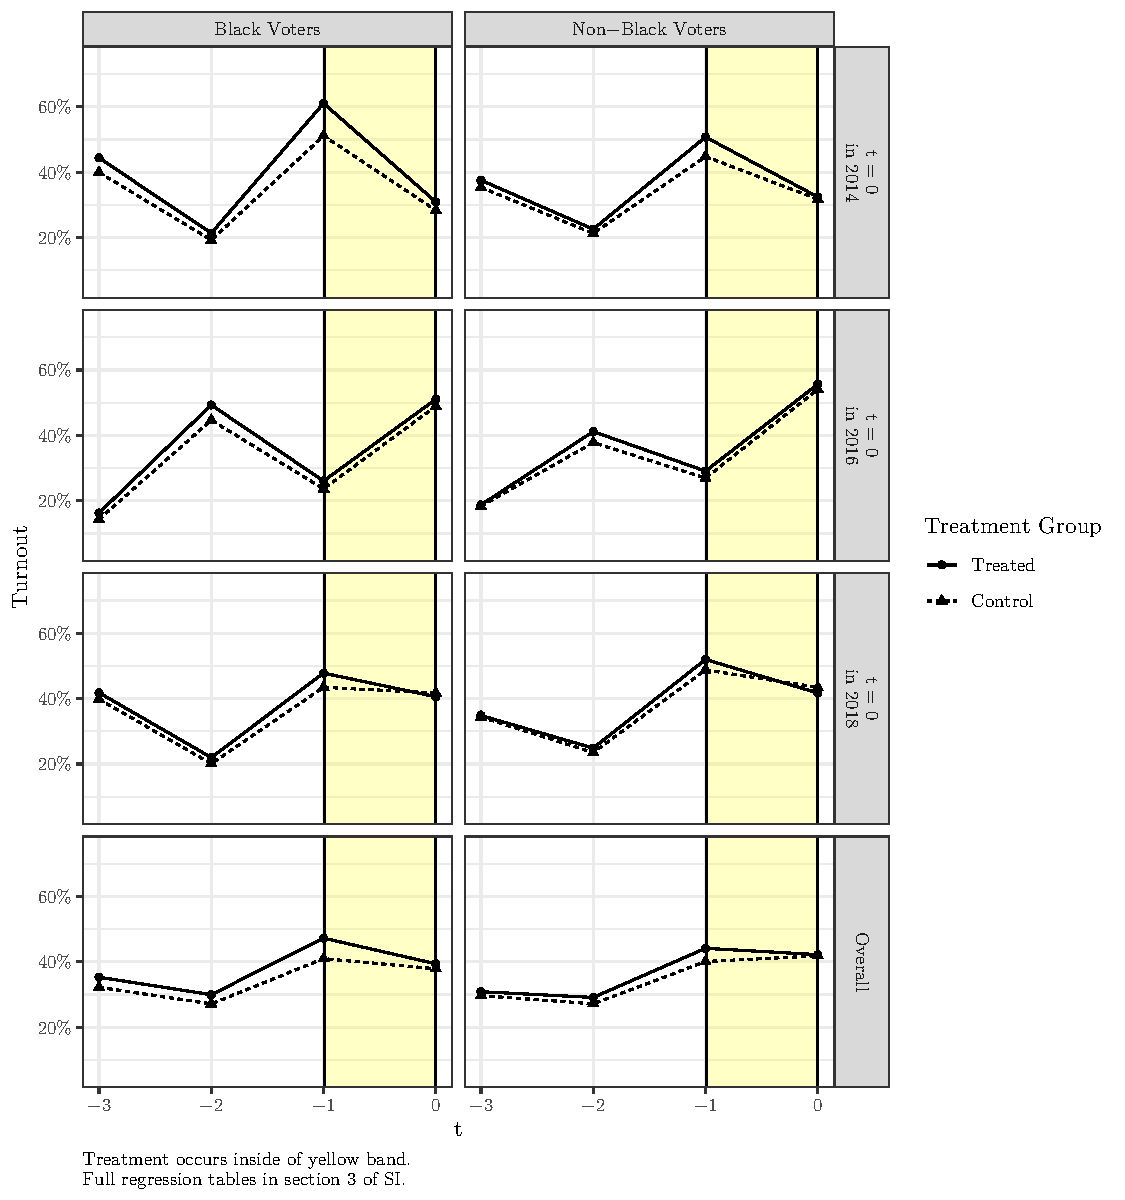
\includegraphics{compile_files/figure-latex/did-no-prior-1} 

}

\caption{\label{fig:did-1}Effect of Being Ticketed on Turnout (no prior turnout in match)}\label{fig:did-no-prior}
\end{figure}

\begin{figure}[H]

{\centering 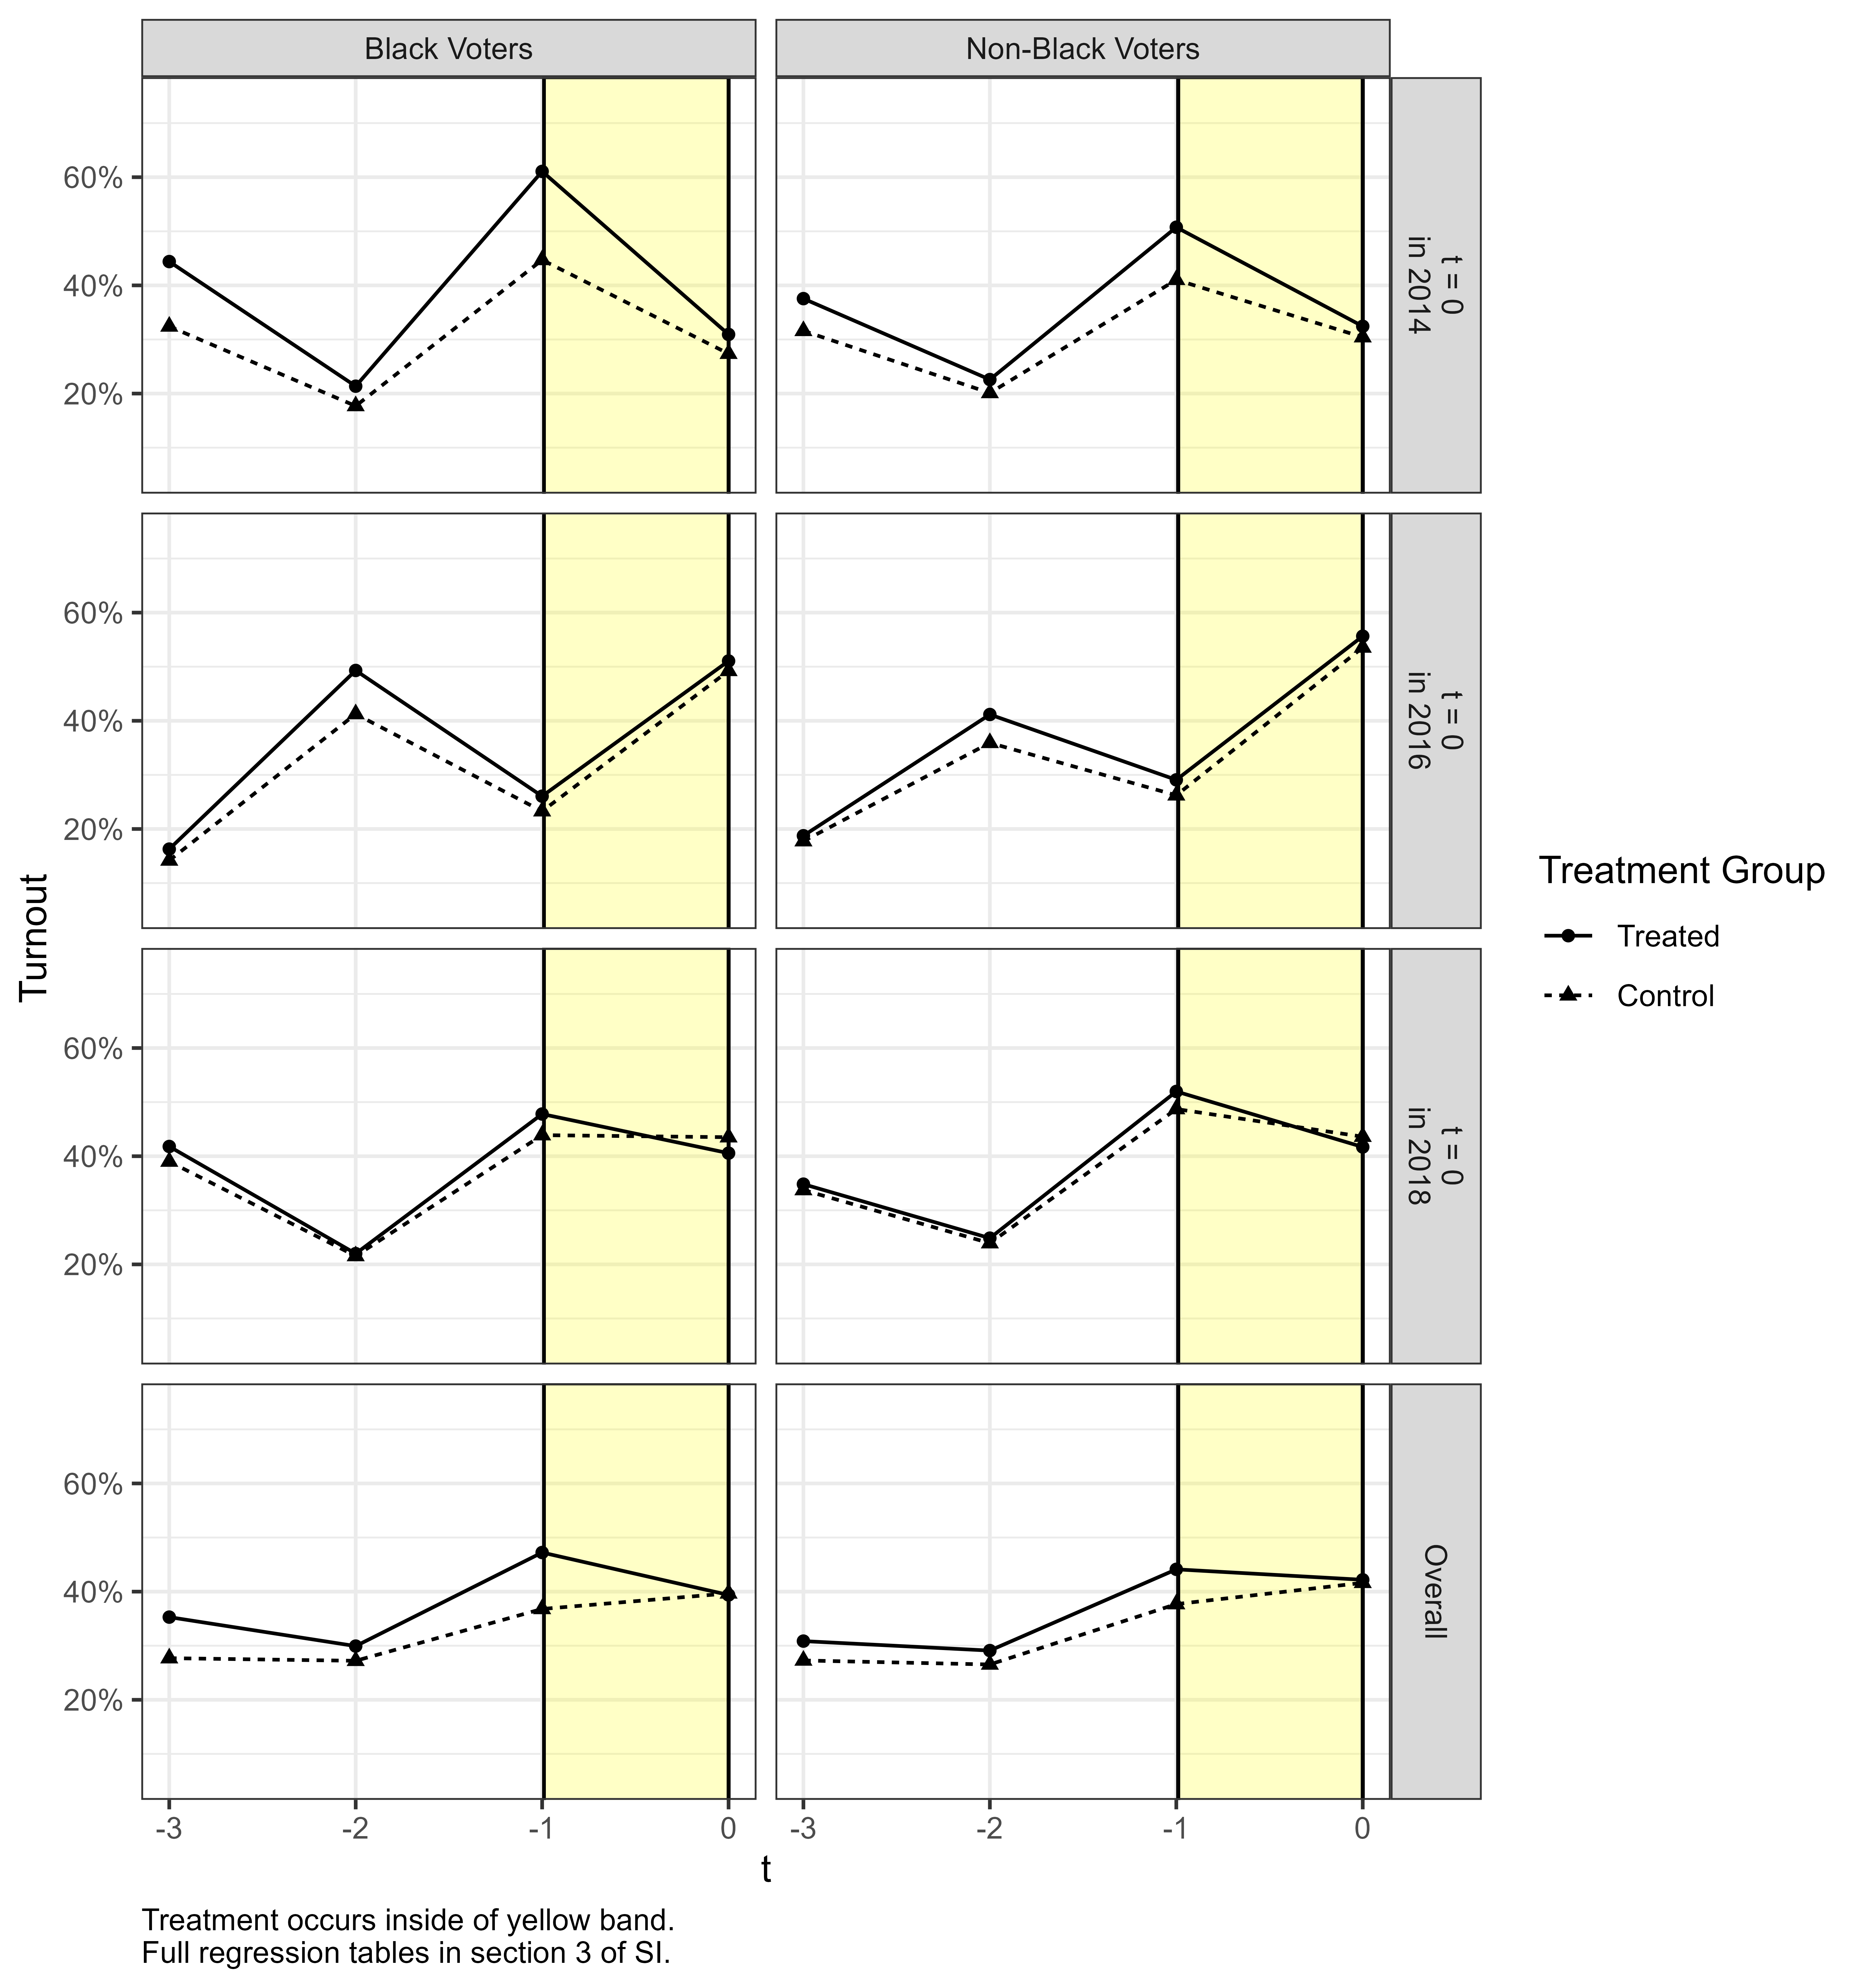
\includegraphics{compile_files/figure-latex/did-no-matching-1} 

}

\caption{\label{fig:did-1}Effect of Being Ticketed on Turnout (no matching at all)}\label{fig:did-no-matching}
\end{figure}

Tables 1--4 are with prior turnout in the match. Tables 5--8 have no prior turnout. Table 9--12 have no matching at all

\begin{singlespace}
\input{"../temp/small_two_matches_reg_overall.tex"}
\input{"../temp/small_two_matches_reg_2014-11-04.tex"}
\input{"../temp/small_two_matches_reg_2016-11-08.tex"}
\input{"../temp/small_two_matches_reg_2018-11-06.tex"}

\input{"../temp/small_table_overall_no_prior.tex"}
\input{"../temp/small_table_2014-11-04_no_prior.tex"}
\input{"../temp/small_table_2016-11-08_no_prior.tex"}
\input{"../temp/small_table_2018-11-06_no_prior.tex"} 

\input{"../temp/small_two_matches_reg_overall_no_matching.tex"}
\input{"../temp/small_two_matches_reg_2014-11-04_no_matching.tex"}
\input{"../temp/small_two_matches_reg_2016-11-08_no_matching.tex"}
\input{"../temp/small_two_matches_reg_2018-11-06_no_matching.tex"}
\end{singlespace}

\begin{figure}[H]

{\centering 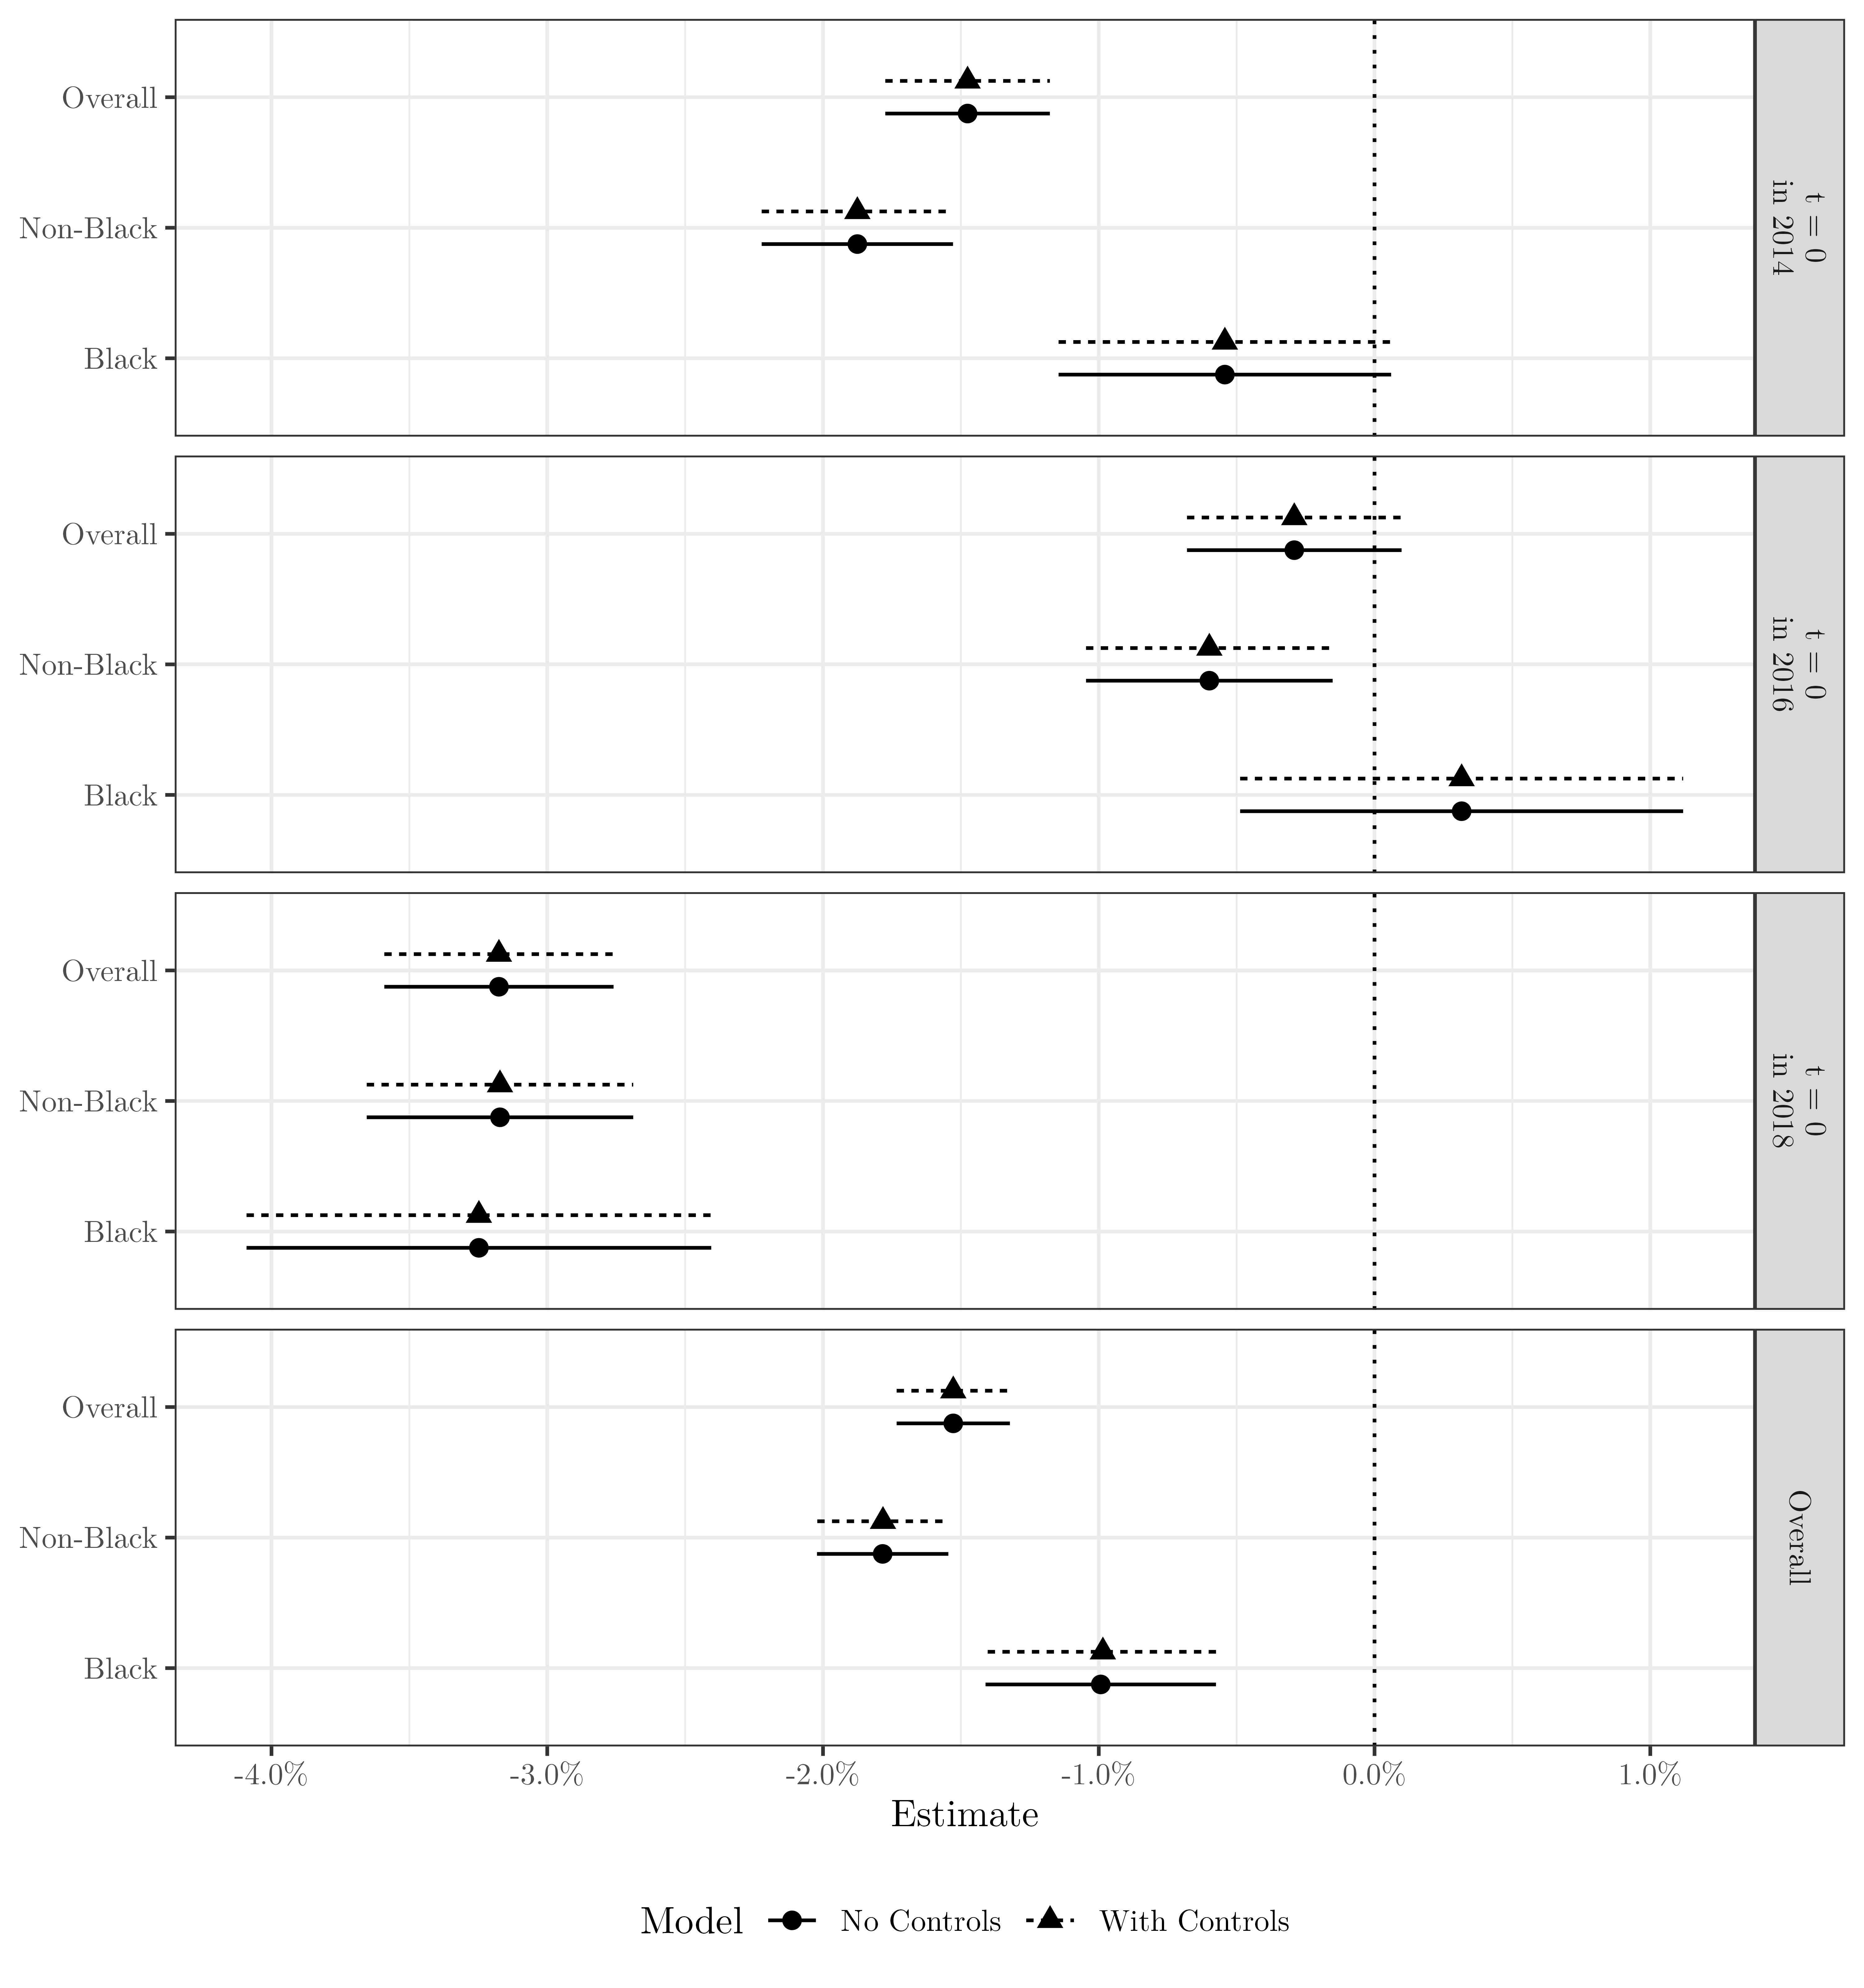
\includegraphics{compile_files/figure-latex/coef-plot-primary-1} 

}

\caption{\label{fig:did-1}Effect of Being Ticketed on Turnout}\label{fig:coef-plot-primary}
\end{figure}

\begin{figure}[H]

{\centering 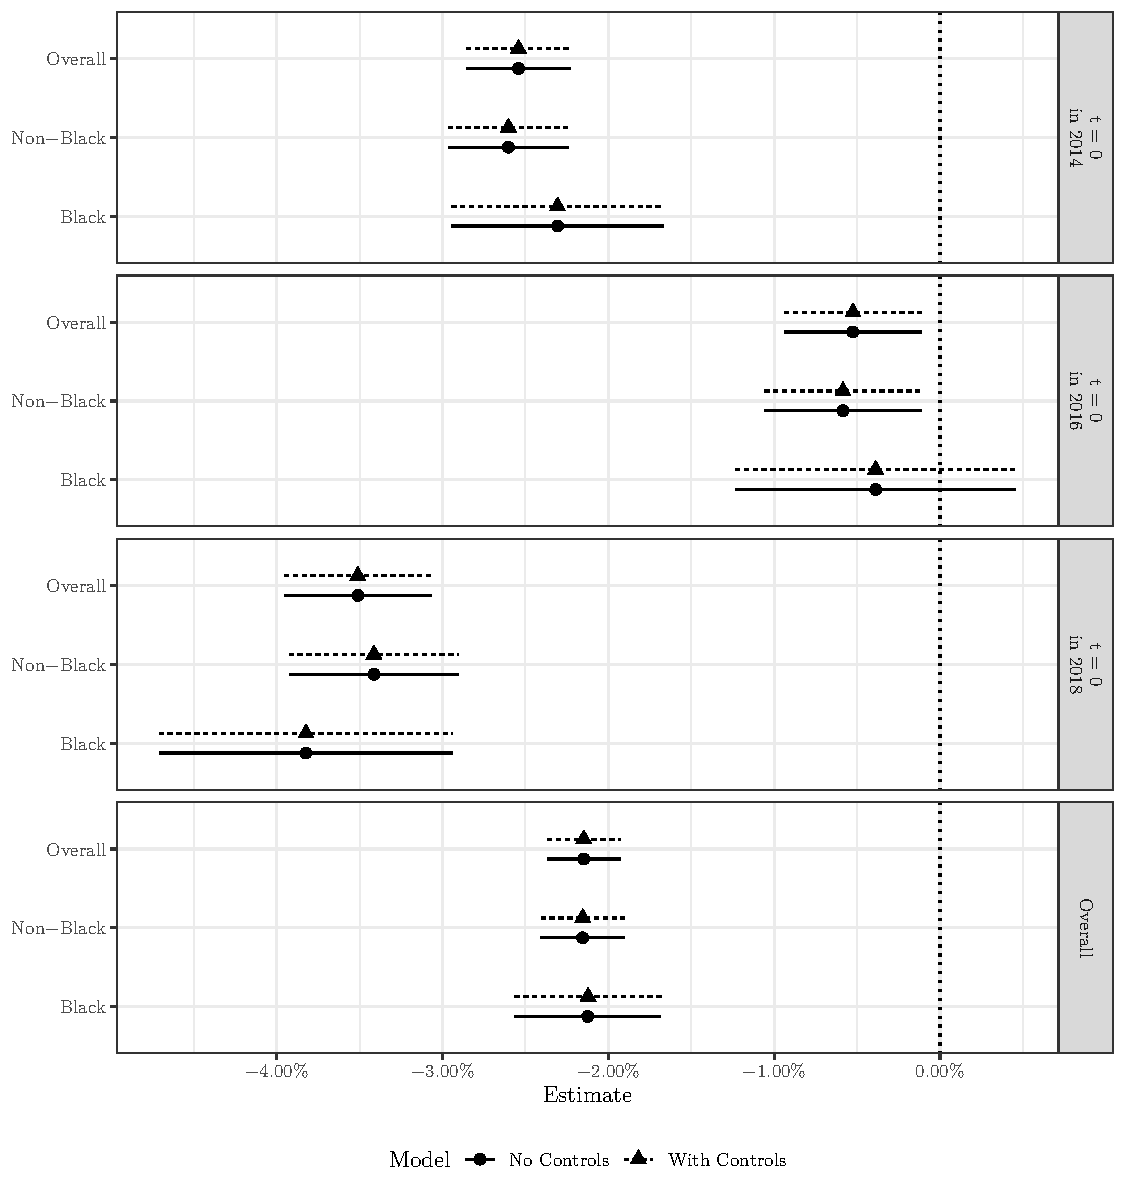
\includegraphics{compile_files/figure-latex/coef-plot-no-prior-1} 

}

\caption{\label{fig:did-1}Effect of Being Ticketed on Turnout (no prior turnout in match)}\label{fig:coef-plot-no-prior}
\end{figure}

\begin{figure}[H]

{\centering 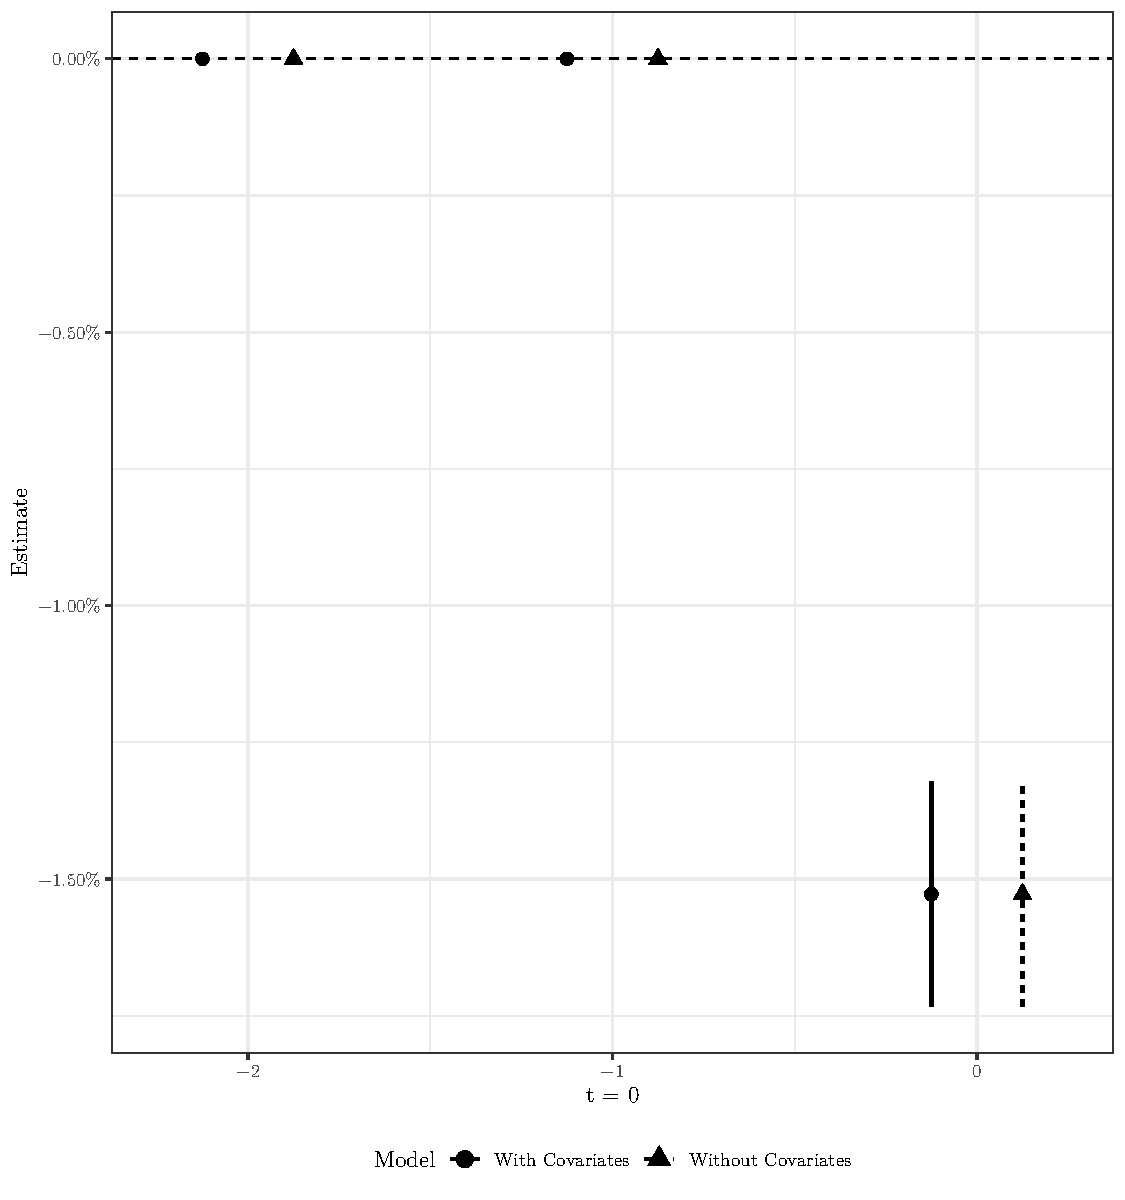
\includegraphics{compile_files/figure-latex/event-study-primary-1} 

}

\caption{\label{fig:did-1}Effect of Being Ticketed on Turnout}\label{fig:event-study-primary}
\end{figure}

\begin{figure}[H]

{\centering 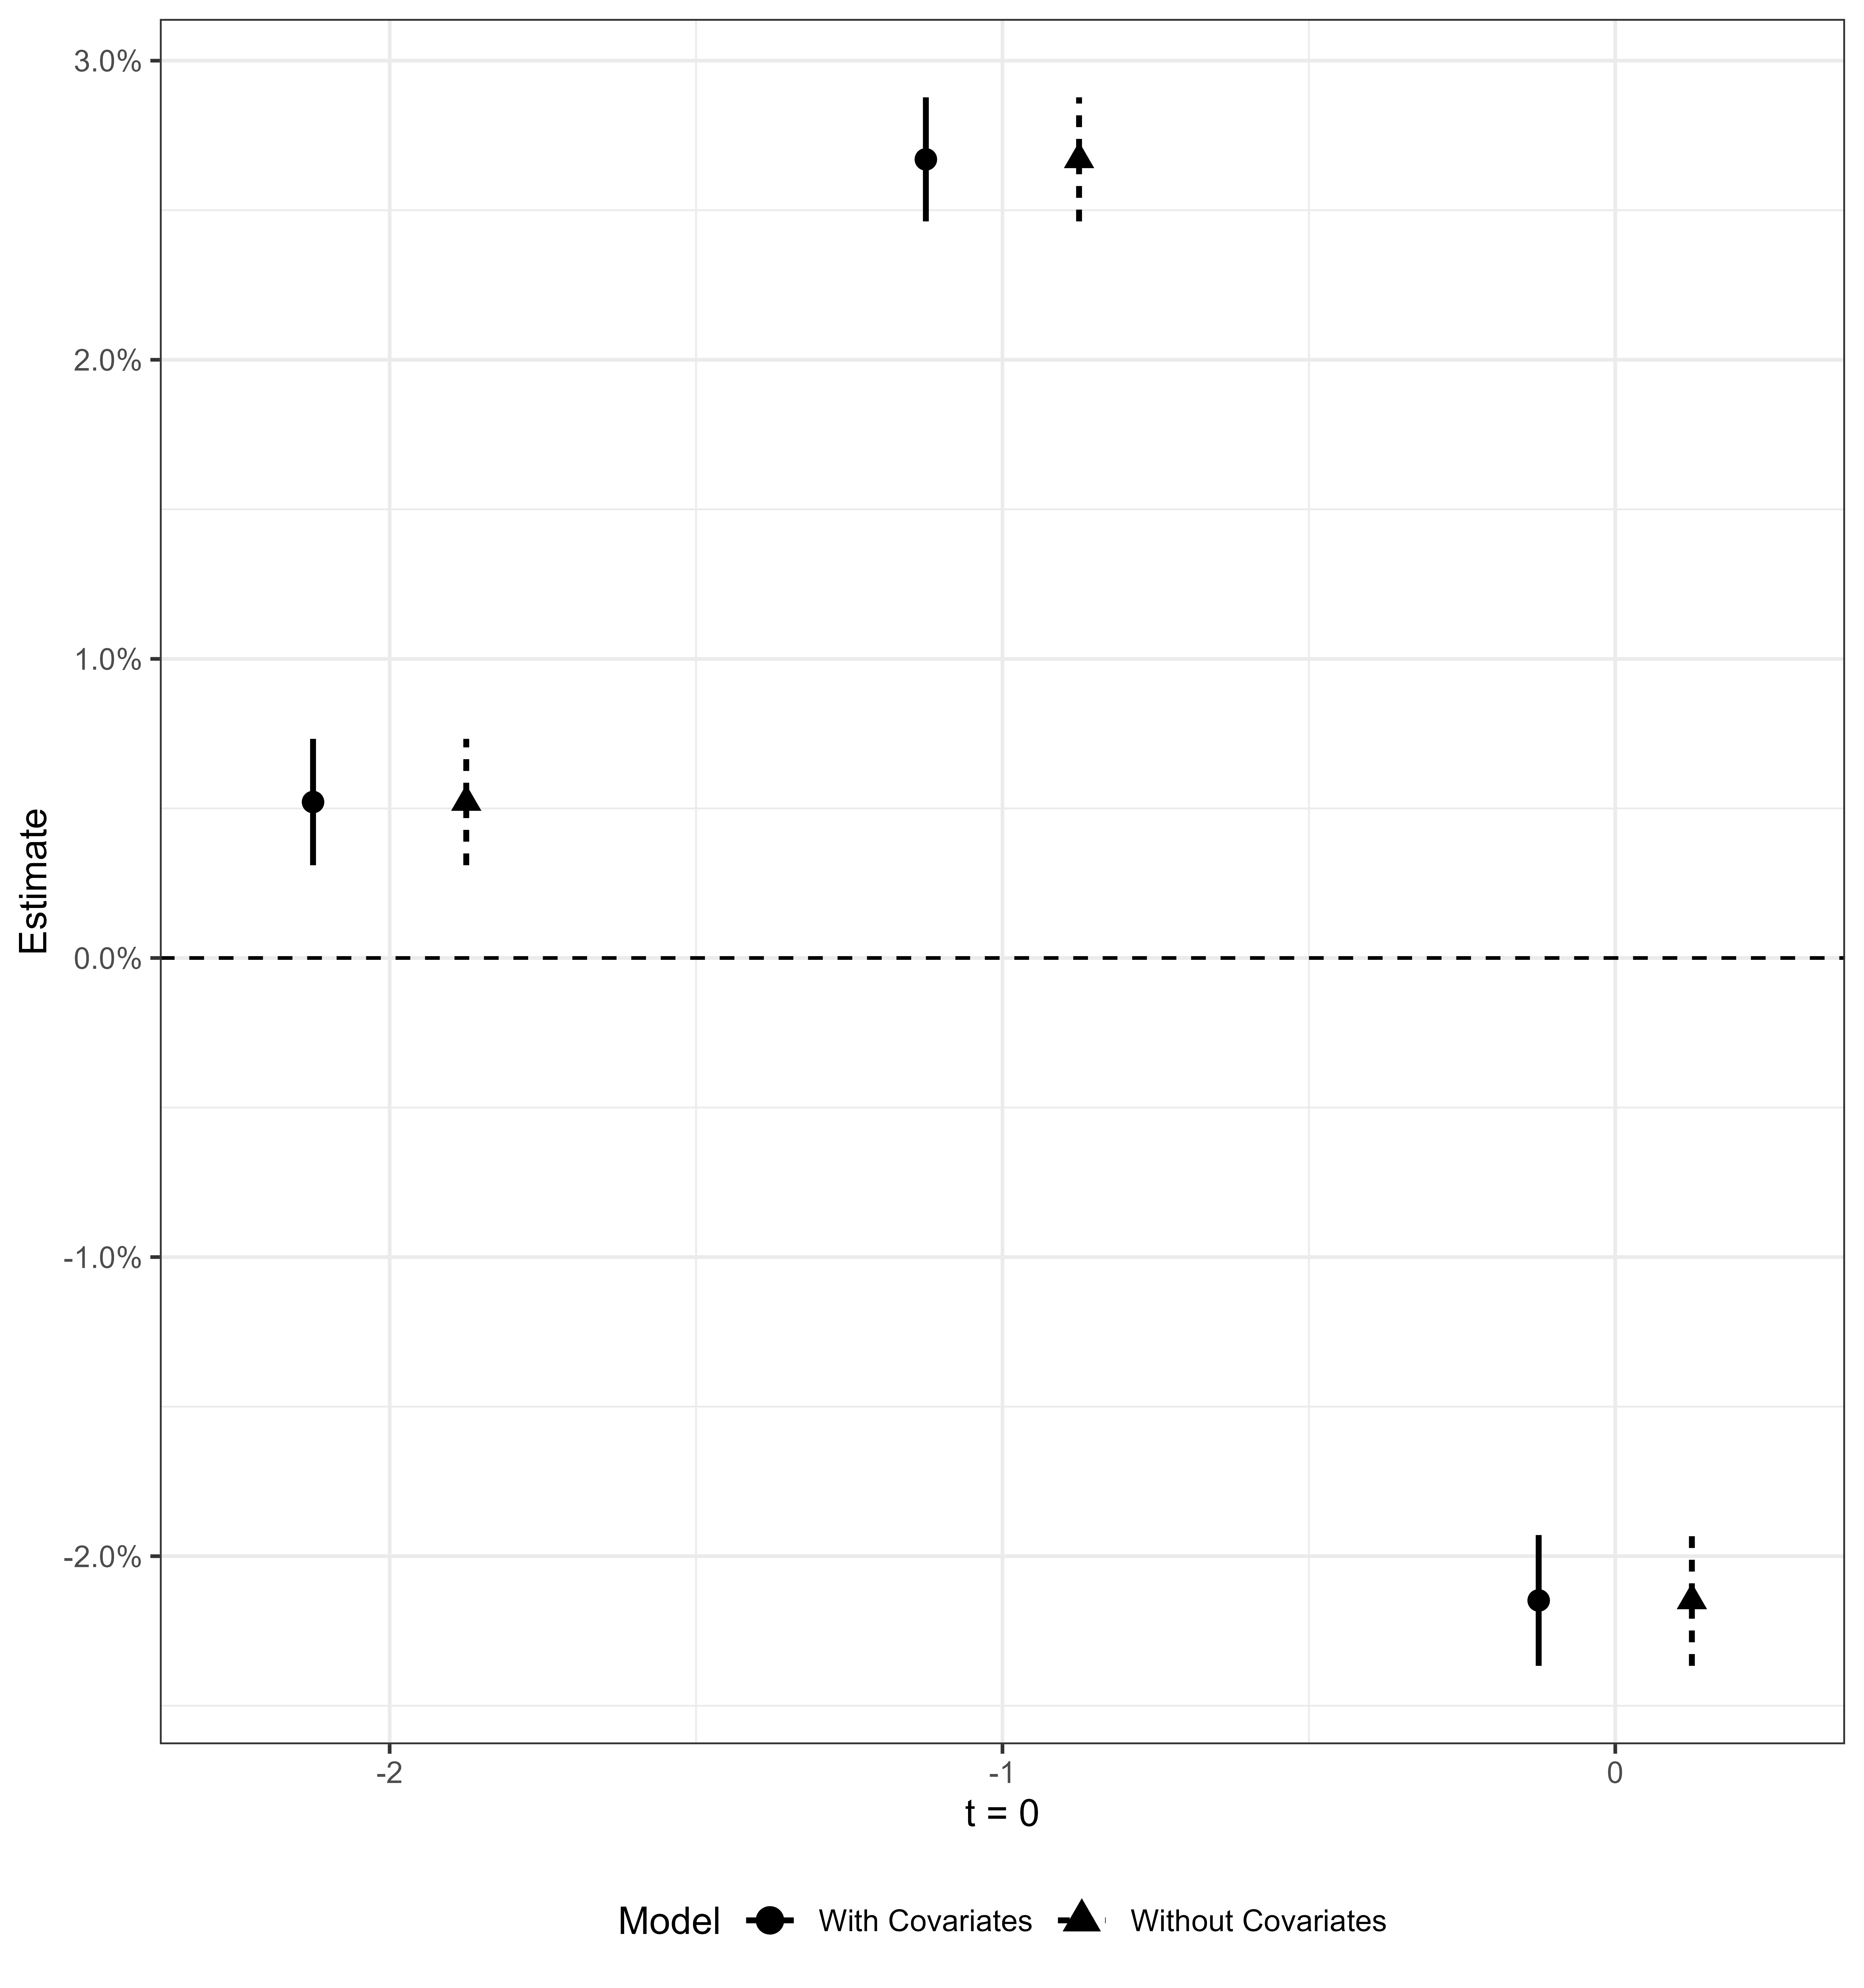
\includegraphics{compile_files/figure-latex/event-study-no-prior-1} 

}

\caption{\label{fig:did-1}Effect of Being Ticketed on Turnout (no prior turnout in match)}\label{fig:event-study-no-prior}
\end{figure}

\begin{figure}[H]

{\centering 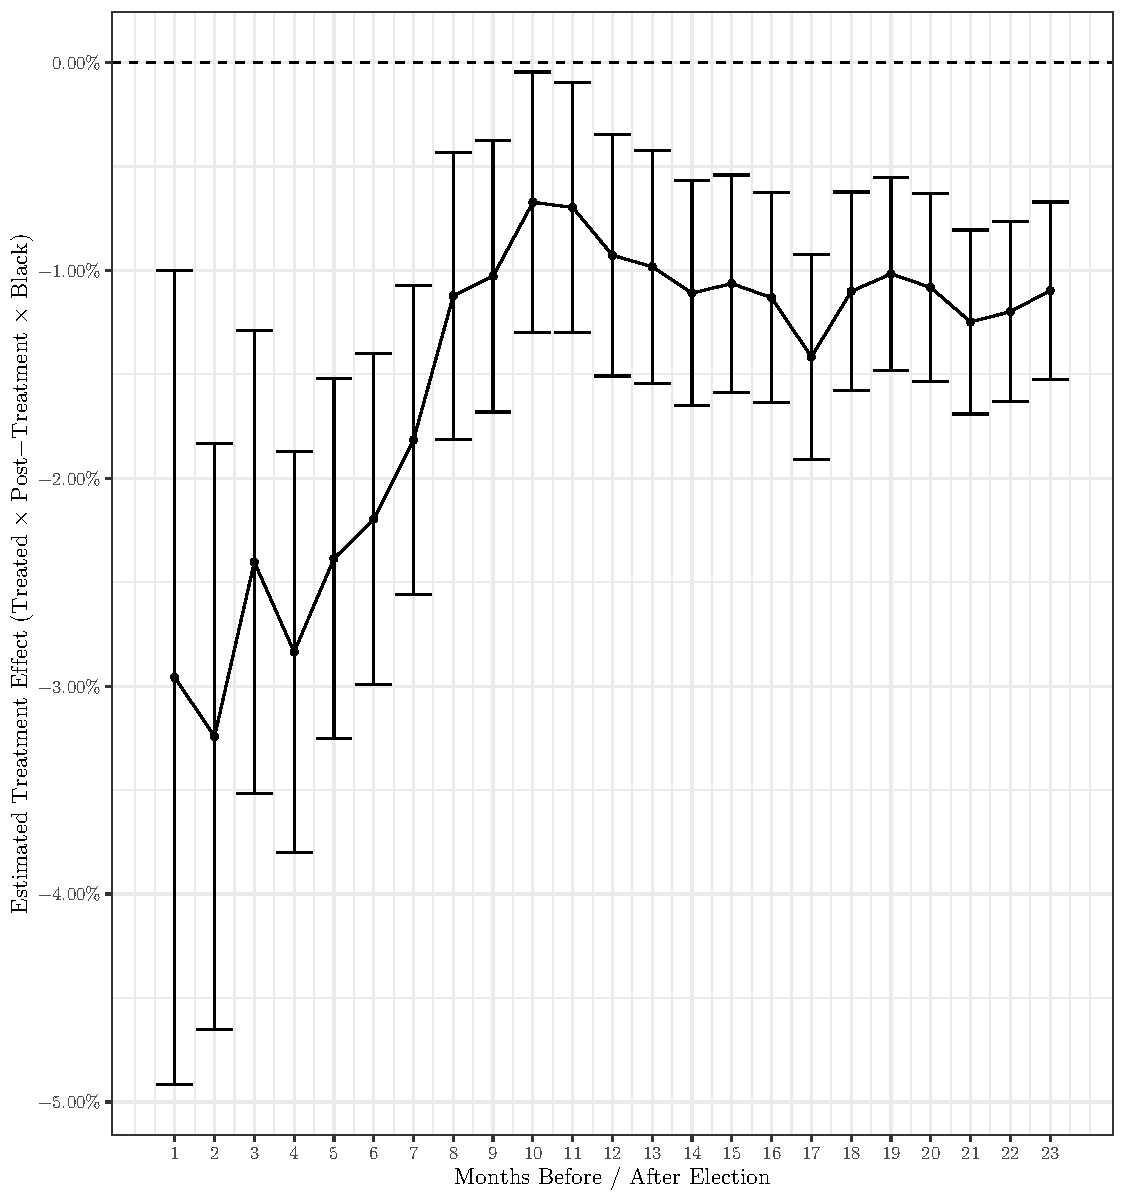
\includegraphics{compile_files/figure-latex/black-overall-primary-1} 

}

\caption{\label{fig:did-1}Black Overall}\label{fig:black-overall-primary}
\end{figure}

\begin{figure}[H]

{\centering 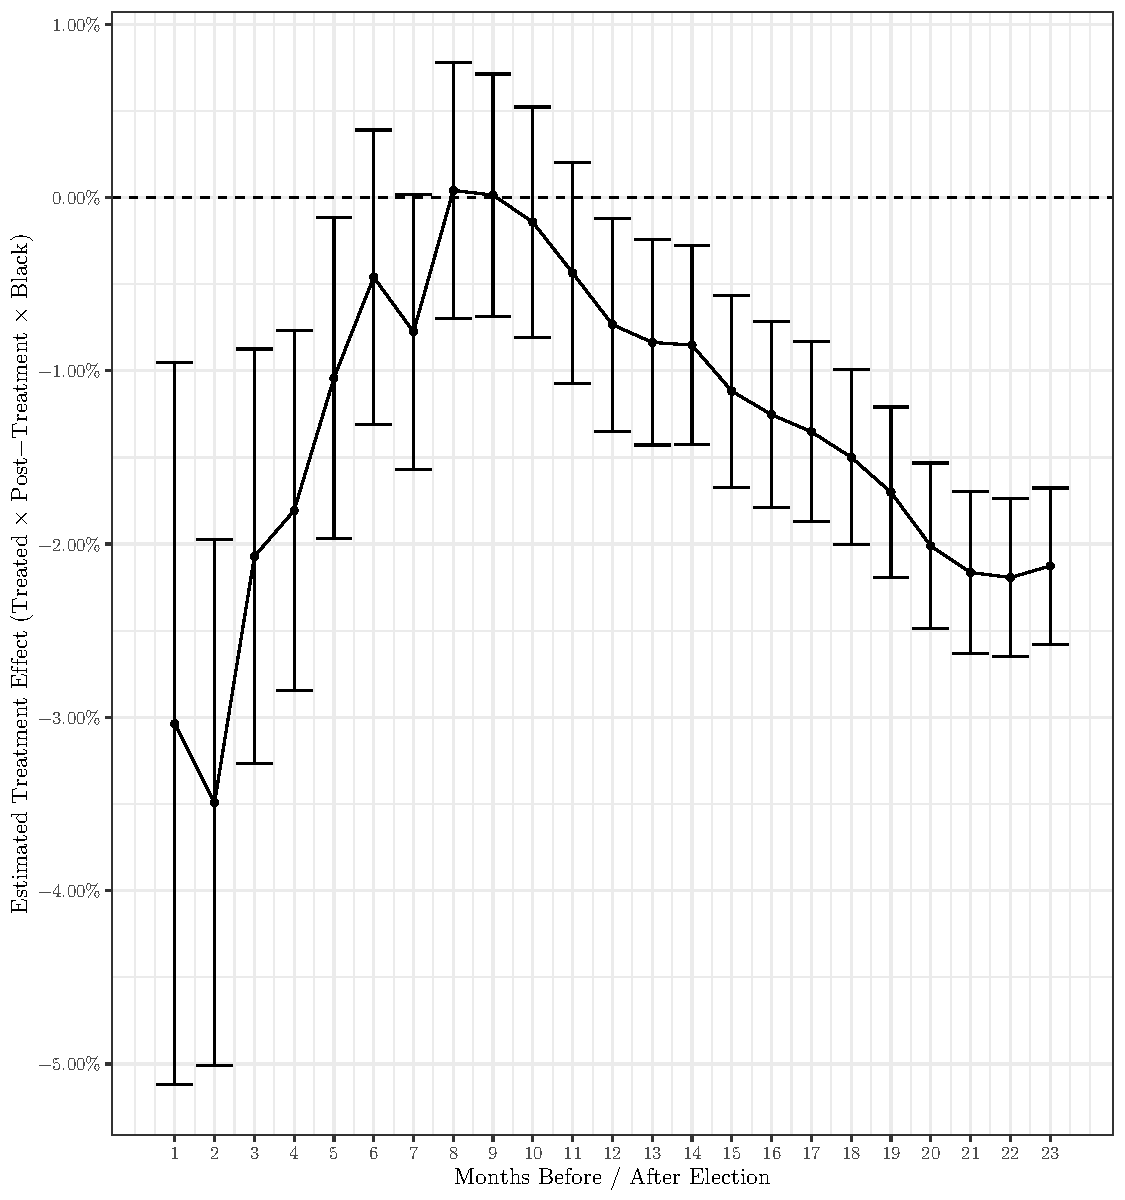
\includegraphics{compile_files/figure-latex/black-overall-no-prior-1} 

}

\caption{\label{fig:did-1}Black Overall (no prior turnout in match)}\label{fig:black-overall-no-prior}
\end{figure}

\begin{figure}[H]

{\centering 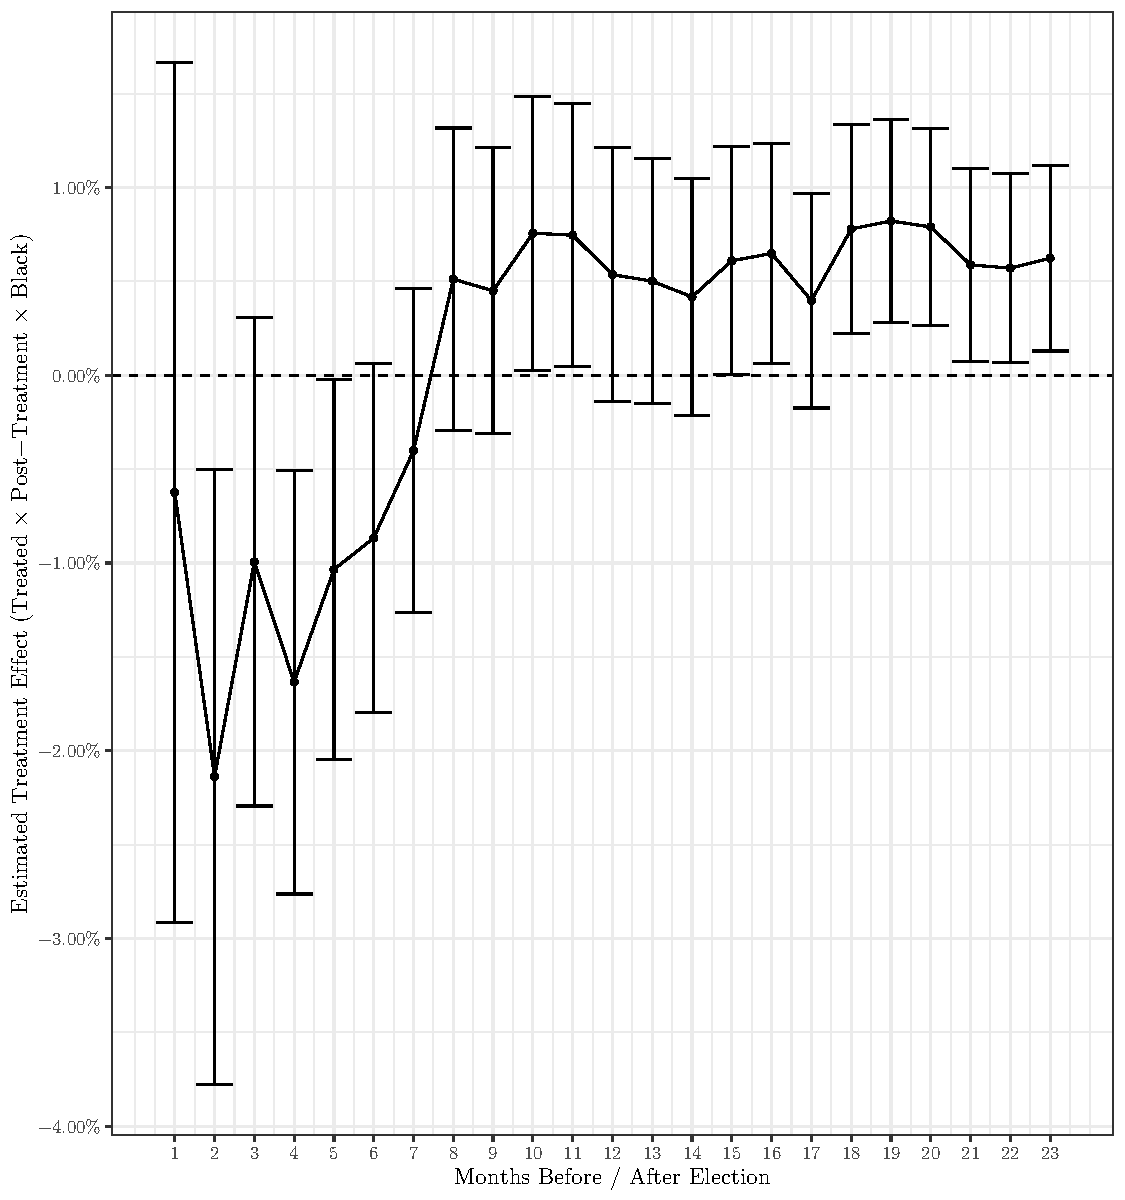
\includegraphics{compile_files/figure-latex/black-relative-primary-1} 

}

\caption{\label{fig:did-1}Black Relative}\label{fig:black-relative-primary}
\end{figure}

\begin{figure}[H]

{\centering 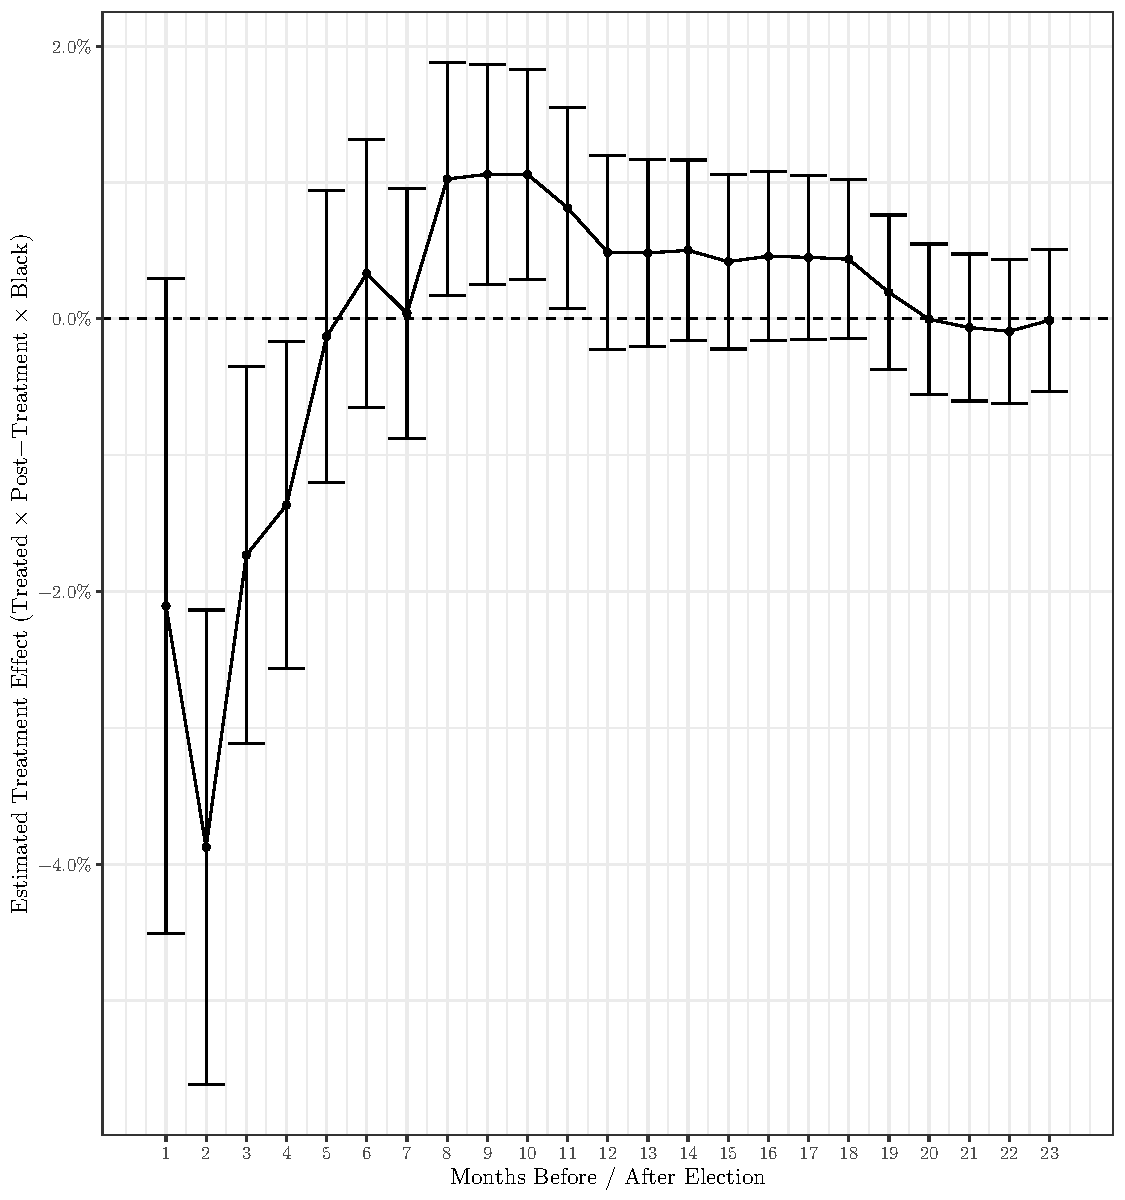
\includegraphics{compile_files/figure-latex/black-relative-no-prior-1} 

}

\caption{\label{fig:did-1}Black Relative (no prior turnout in match)}\label{fig:black-relative-no-prior}
\end{figure}

\begin{figure}[H]

{\centering 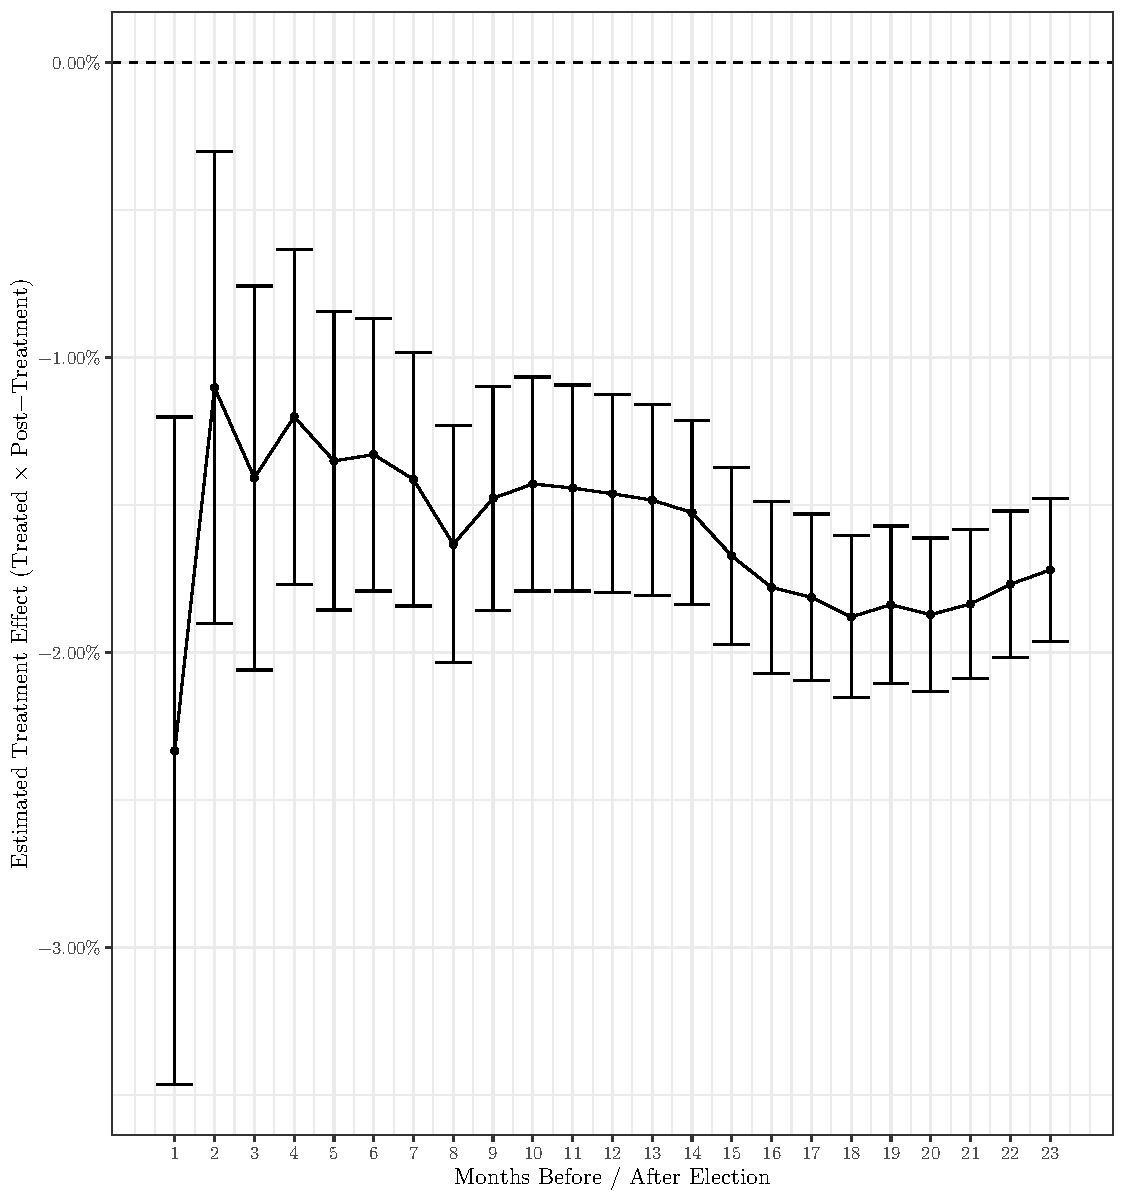
\includegraphics{compile_files/figure-latex/non-black-primary-1} 

}

\caption{\label{fig:did-1}Nonblack}\label{fig:non-black-primary}
\end{figure}

\begin{figure}[H]

{\centering 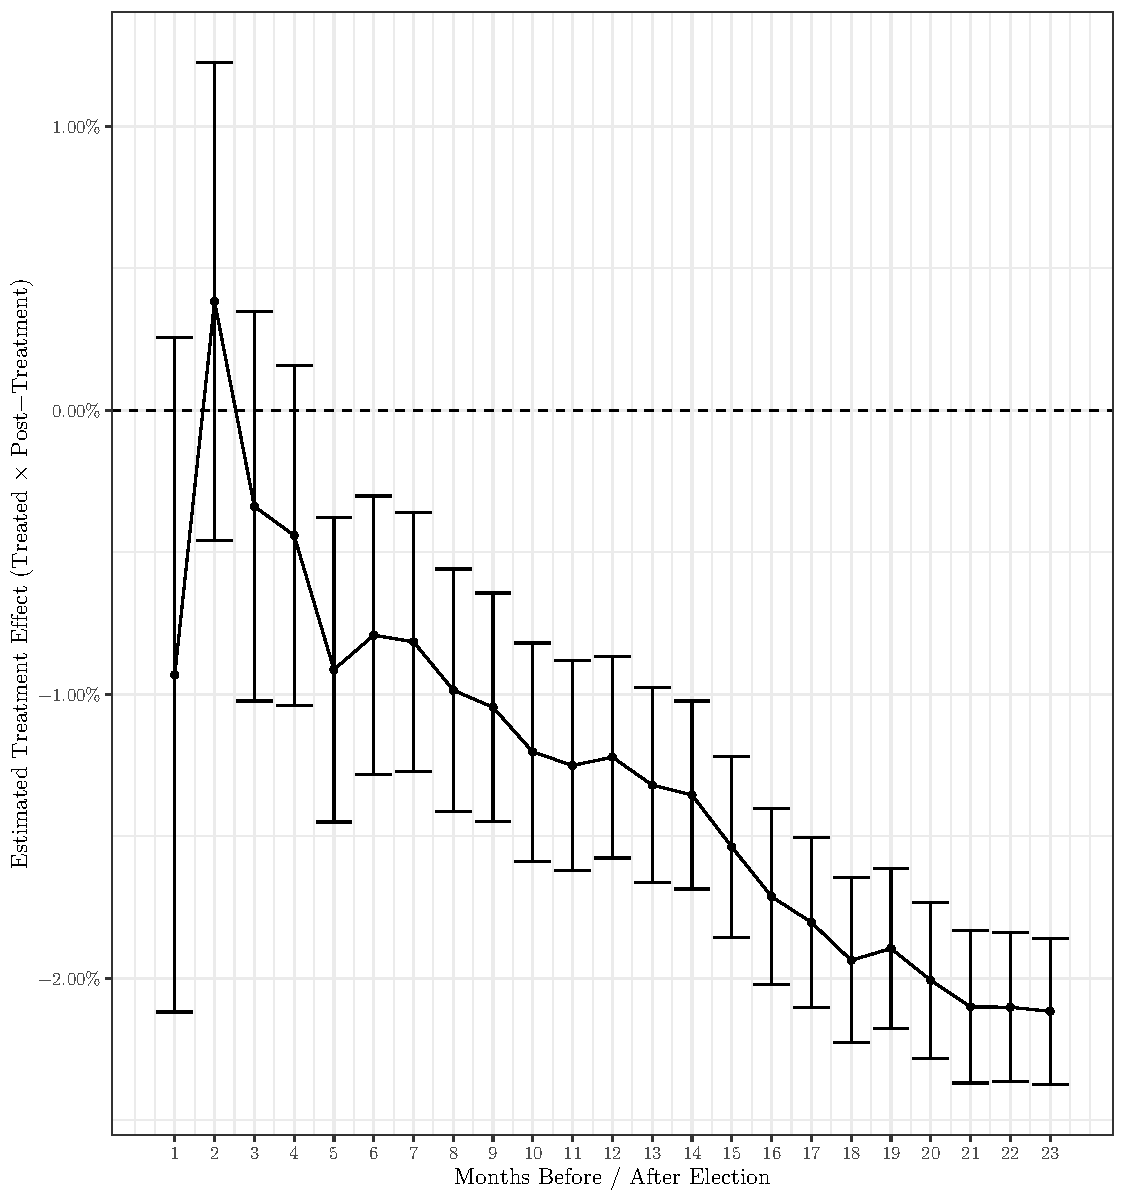
\includegraphics{compile_files/figure-latex/non-black-no-prior-1} 

}

\caption{\label{fig:did-1}Nonblack (no prior turnout in match)}\label{fig:non-black-no-prior}
\end{figure}

\begin{figure}[H]

{\centering 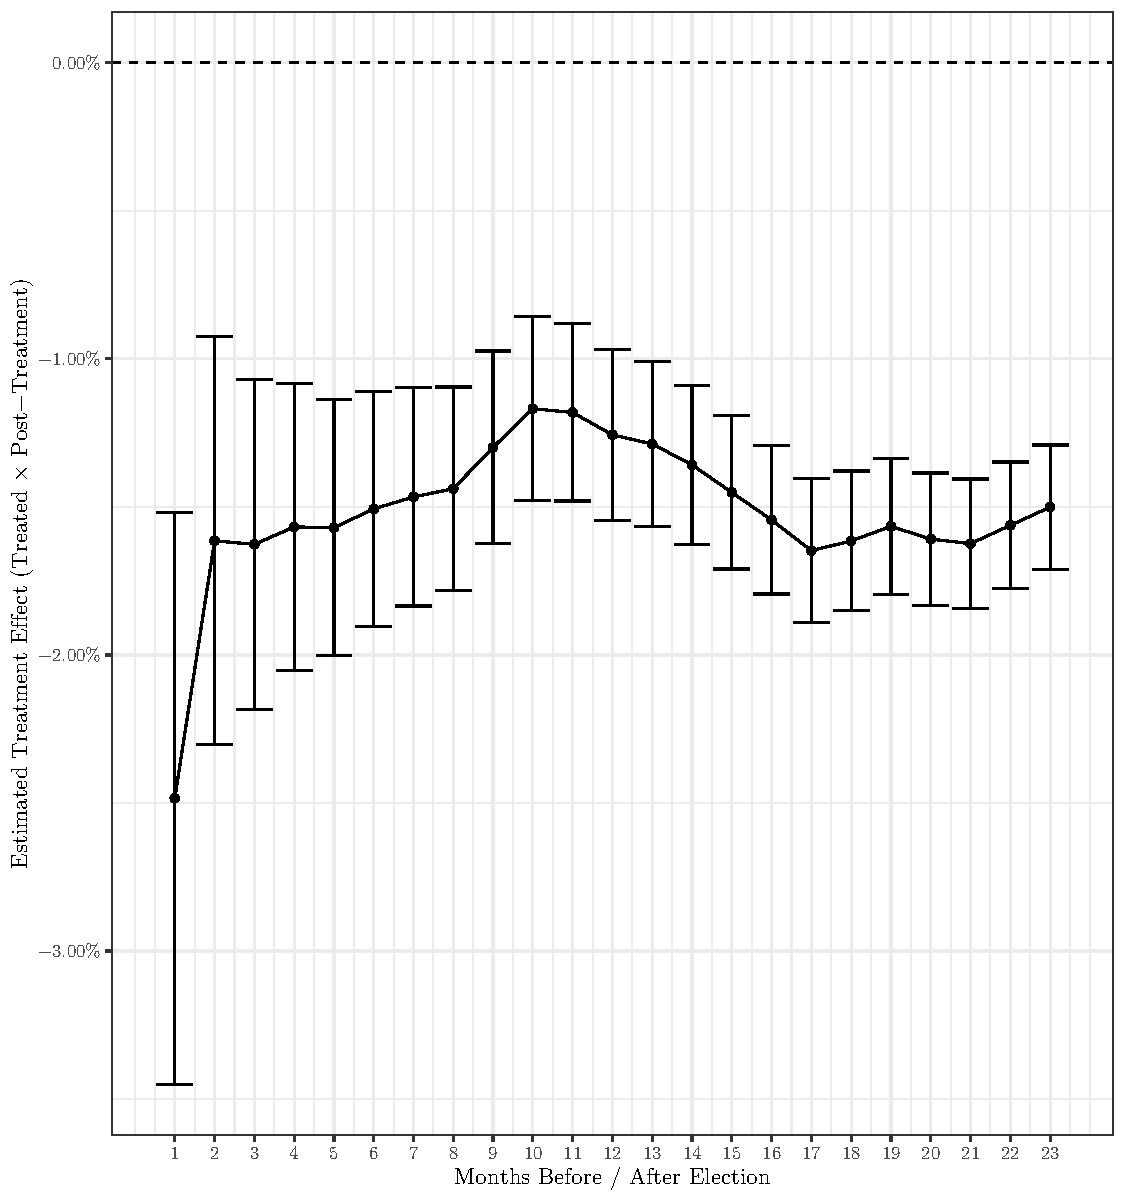
\includegraphics{compile_files/figure-latex/overall-time-primary-1} 

}

\caption{\label{fig:did-1}Black Relative}\label{fig:overall-time-primary}
\end{figure}

\begin{figure}[H]

{\centering 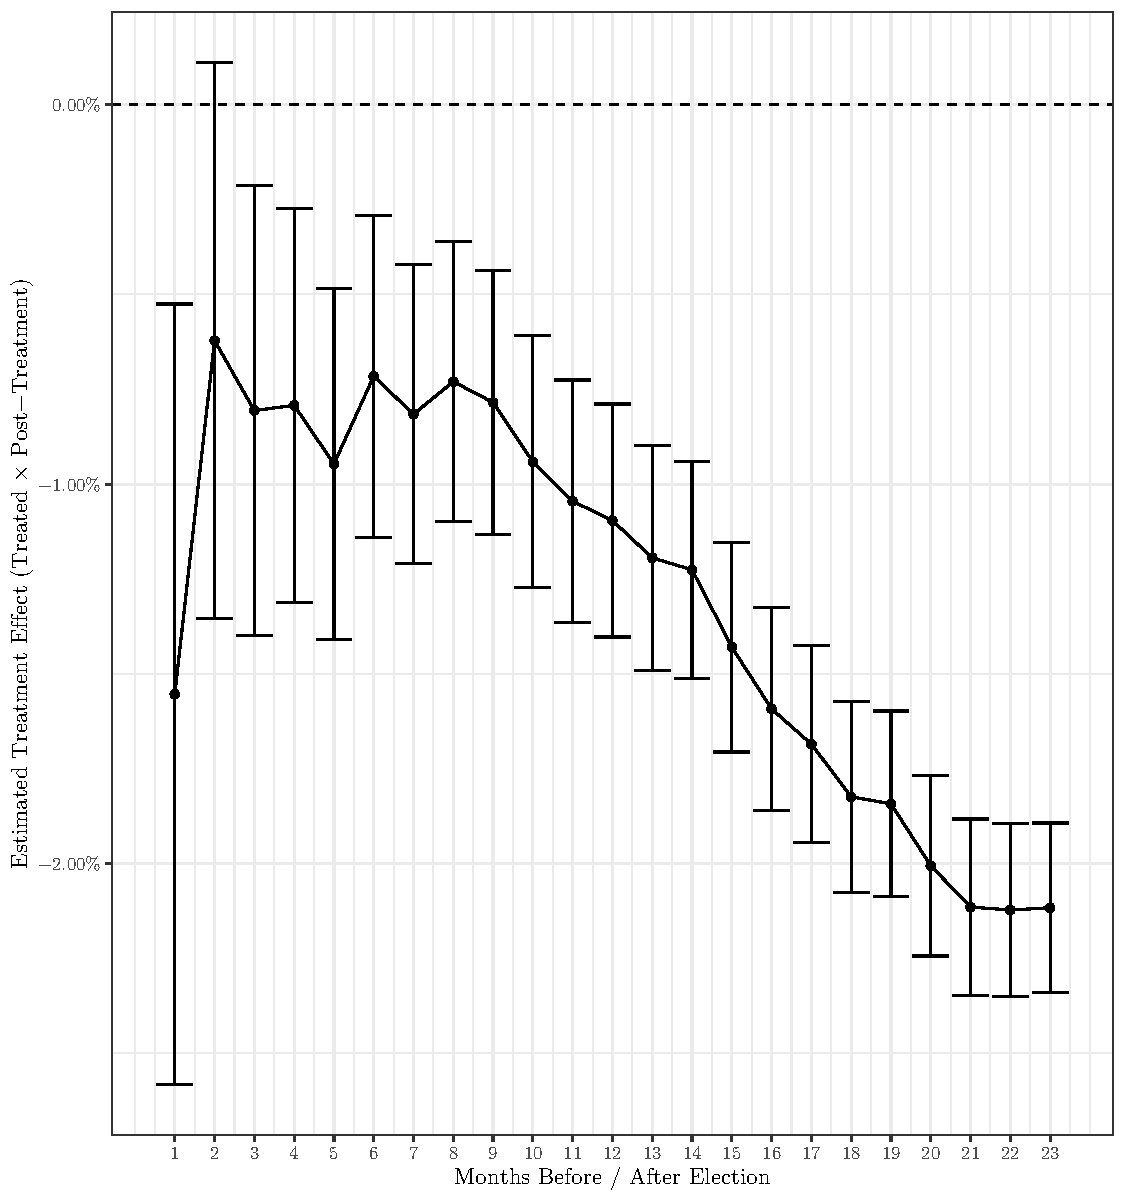
\includegraphics{compile_files/figure-latex/overall-time-no-prior-1} 

}

\caption{\label{fig:did-1}Black Relative (no prior turnout in match)}\label{fig:overall-time-no-prior}
\end{figure}

\end{document}
